%! alt Square ABCD with side 10, AB along the bottom and CD along the top. A circle through A and B touches CD at T, the midpoint of CD, with a right angle between the radius OT and CD. The centre O is at height k above the midpoint N of AB. The radii OA and OT both have length r, and triangle ANO is right-angled, with AN = 5 and NO = k.
%! after_paragraph 1
%! scale 3/5
% The shared preamble of every Kyuclid figure. pipeline/figures turns these colours into theme-aware paint,
% and refuses any other colour, so draw only with them:
%   figink (lines and labels), figaux (construction lines), figaccent (the object the argument turns on),
%   figtint and figaccenttint (light fills).
\documentclass[border=1.5pt]{standalone}
\usepackage{tkz-euclide}
\definecolor{figink}{RGB}{0,0,0}
\definecolor{figaux}{RGB}{85,85,85}
\definecolor{figaccent}{RGB}{192,57,43}
\definecolor{figtint}{RGB}{221,221,221}
\definecolor{figaccenttint}{RGB}{245,213,208}
% tkz-euclide's defaults draw circles, compasses and marks in 50% grey and fill points with a tint.
\makeatletter
\def\tkz@otherlinecolor{figink}
\def\tkz@euc@circlecolor{figink}
\def\tkz@euc@compasscolor{figink}
\def\tkz@euc@mkcolor{figink}
\def\tkz@mk@fill{figink}
\def\tkz@euc@pointfillcolor{figink}
\makeatother
\tkzSetUpLine[color=figink,line width=.7pt]
\tkzSetUpArc[color=figink,line width=.7pt]
\tkzSetUpCompass[color=figink,line width=.5pt]
\tkzSetUpPoint[color=figink,fill=figink,size=3.1pt]
\tikzset{
  every picture/.style={line cap=round,line join=round,color=figink},
  circle style/.append style={color=figink,line width=.7pt},
  aux/.style={color=figaux,line width=.45pt,dash pattern=on 2.6pt off 2pt},
  key/.style={color=figaccent,line width=1pt},
  mk/.style={color=figink,line width=.5pt},
  lbl/.style={color=figink,inner sep=2.2pt},
  len/.style={color=figink,inner sep=1.5pt,font=\small},
}

\begin{document}
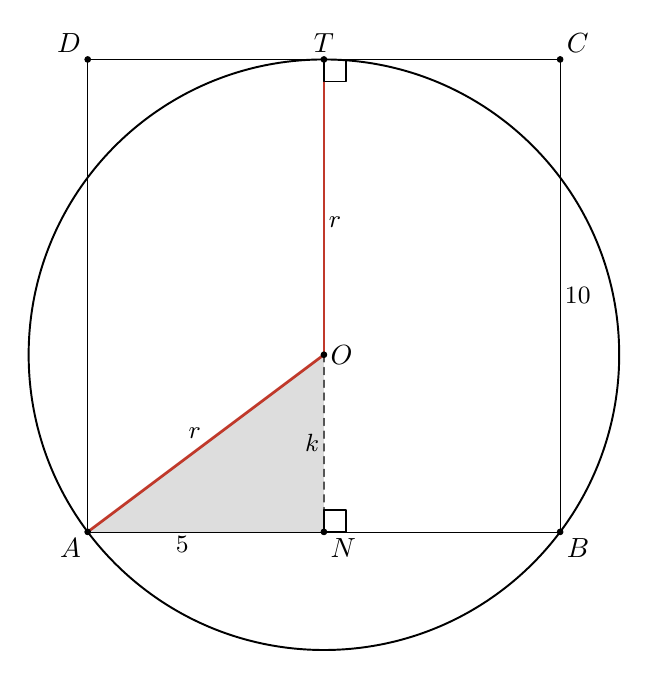
\begin{tikzpicture}
\tkzDefPoint(0.0,0.0){A} %! A = (0, 0)
\tkzDefPoint(6.0000000,0.0){B} %! B = (10, 0)
\tkzDefPoint(6.0000000,6.0000000){C} %! C = (10, 10)
\tkzDefPoint(0.0,6.0000000){D} %! D = (0, 10)
\tkzDefPoint(3.0000000,2.2500000){O} %! O = (5, 15/4)
\tkzDefPoint(3.0000000,6.0000000){T} %! T = (5, 10)
\tkzDefPoint(3.0000000,0.0){N} %! N = mid(A, B)
%! fact dist(A, B) == 10
%! fact dist(B, C) == 10
%! fact perp(A, B, B, C)
%! fact on_circle(A, O, 25/4)
%! fact on_circle(B, O, 25/4)
%! fact tangent(O, 25/4, C, D)
%! fact on_circle(T, O, 25/4)
%! fact on_segment(T, C, D)
%! fact dist(N, O) == 15/4
\tkzFillPolygon[color=figtint](A,N,O)
\tkzDrawCircle(O,T)
\tkzDrawPolygon(A,B,C,D)
\tkzDrawSegment[aux](O,N)
\tkzDrawSegment[key](O,T)
\tkzDrawSegment[key](O,A)
\tkzMarkRightAngle[size=.28,mk](O,T,C)
\tkzMarkRightAngle[size=.28,mk](O,N,B)
\tkzDrawPoints(A,B,C,D,O,T,N)
\tkzLabelPoint[below left,lbl](A){$A$}
\tkzLabelPoint[below right,lbl](B){$B$}
\tkzLabelPoint[above right,lbl](C){$C$}
\tkzLabelPoint[above left,lbl](D){$D$}
\tkzLabelPoint[above,lbl](T){$T$}
\tkzLabelPoint[below right,lbl](N){$N$}
\tkzLabelPoint[right,lbl](O){$O$}
\tkzLabelSegment[right,pos=.45,len](O,T){$r$}
\tkzLabelSegment[above left,len](A,O){$r$}
\tkzLabelSegment[below,pos=.4,len](A,N){$5$}
\tkzLabelSegment[left,len](O,N){$k$}
\tkzLabelSegment[right,len](B,C){$10$}
\end{tikzpicture}
\end{document}
